\documentclass[onecolumn]{article}
%\usepackage{url}
%\usepackage{algorithmic}
\usepackage[a4paper]{geometry}
\usepackage{datetime}
\usepackage[margin=2em, font=small,labelfont=it]{caption}
\usepackage{graphicx}
\usepackage{mathpazo} % use palatino
\usepackage[scaled]{helvet} % helvetica
\usepackage{microtype}
\usepackage{amsmath}
\usepackage{subfigure}
% Letterspacing macros
\newcommand{\spacecaps}[1]{\textls[200]{\MakeUppercase{#1}}}
\newcommand{\spacesc}[1]{\textls[50]{\textsc{\MakeLowercase{#1}}}}

\title{\spacecaps{Data Mining Final Project: Predicting Mental Health Illnesses In Tech Workplace}\\ \normalsize \spacesc{CENG 3521, Data Mining} }

\author{Ayhan Yüksek - Ümit Kadiroğlu\\ayhanyuksek@posta.mu.edu.tr - umitkadiroglu@posta.mu.edu.tr}



%\date{\today\\\currenttime}
\date{\today}

\begin{document}
\maketitle
\textbf{GitHub account}: https://github.com/ayhanyuksek/DataMiningFinalProject


\section{Introduction}
In this project, we found a dataset about mental health in tech workplace. The dataset contains the results of the survey applied in 2014. The survey asks the following data:
\begin{itemize}
\item Timestamp
\item Age
\item Gender
\item Country
\item state: If you live in the United States, which state or territory do you live in?
\item self\_employed: Are you self-employed?
\item family\_history: Do you have a family history of mental illness?
\item treatment: Have you sought treatment for a mental health condition?
\item work\_interfere: If you have a mental health condition, do you feel that it interferes with your work?
\item no\_employees: How many employees does your company or organization have?
\item remote\_work: Do you work remotely (outside of an office) at least 50% of the time?
\item tech\_company: Is your employer primarily a tech company/organization?
\item benefits: Does your employer provide mental health benefits?
\item care\_options: Do you know the options for mental health care your employer provides?
\item wellness\_program: Has your employer ever discussed mental health as part of an employee wellness program?
\item seek\_help: Does your employer provide resources to learn more about mental health issues and how to seek help?
\item anonymity: Is your anonymity protected if you choose to take advantage of mental health or substance abuse treatment resources?
\item leave: How easy is it for you to take medical leave for a mental health condition?
\item mental\_health\_consequence: Do you think that discussing a mental health issue with your employer would have negative consequences?
\item phys\_health\_consequence: Do you think that discussing a physical health issue with your employer would have negative consequences?
\item coworkers: Would you be willing to discuss a mental health issue with your coworkers?
\item supervisor: Would you be willing to discuss a mental health issue with your direct supervisor(s)?
\item mental\_health\_interview: Would you bring up a mental health issue with a potential employer in an interview?
\item phys\_health\_interview: Would you bring up a physical health issue with a potential employer in an interview?
\item mental\_vs\_physical: Do you feel that your employer takes mental health as seriously as physical health?
\item obs\_consequence: Have you heard of or observed negative consequences for coworkers with mental health conditions in your workplace?
\item comments: Any additional notes or comments
\end{itemize}

Our main purpose was to predict whether a patient needs treatment or not, using the values from the dataset. In supervised learning part; we went through certain processes, such as cleaning our dataset from null values and encoding to make our dataset suitable for training algorithms. Then we made some visualizations and aimed to realize the correlations between the data and to have a general impression of the participants in our dataset. After all, we started to tune our algorithms to learn the best parameters. We trained and predicted using with these parameters. Finally, we compared the accuracy of these algorithms and determined the best one.


\section{Supervised Learning}
Supervised learning is the machine learning task of learning a function that maps an input to an output based on example input-output pairs [1]. In this project, we have pre-processed our dataset for the supervised learning part. Then, by visualizing our dataset, we aimed to understand our dataset better and to find the correlations between data. Finally, we compared models using various supervised algorithms, such as Logistic Regression, AdaBoost Classifier, KNeighbors Classifier, Random Forest Classifier, Bagging Classifier and tried to find the one with the highest success rate.

\subsection{Data Pre-processing}
Data pre-processing is a data mining technique which is used to transform the raw data in a useful and efficient format [2]. After we loaded our dataset, we cleaned it with several processes and finally encoded it.

\subsubsection{Loading dataset}
We have loaded our ".csv" type dataset by importing the Pandas package. Then we printed the shape and feature names of our dataset as shown in Figure 1.

\begin{figure}[h]
\centering
    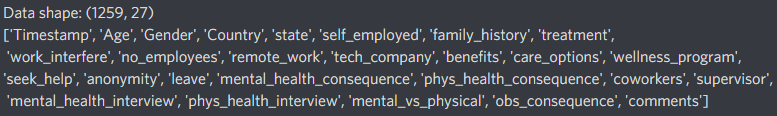
\includegraphics[width=.8\linewidth]{fig/fig1.png}
\caption{\label{figure1}
Data shape and features.}
\end{figure}

\subsubsection{Cleaning our dataset}
We deleted the columns in the dataset that we did not think would affect the result and corrected the unassigned, uncategorized and illogical values. We performed these operations in 7 parts.\bigbreak

\textbf{\emph{Part 1: Deleting some of the features that we don't want to use}}\bigbreak
We deleted "Timestamp", "state", "comments", "Country", "{tech\_company}" and "{obs\_consequences}" columns that contains unnecessary and irrelevant data.\bigbreak

\textbf{\emph{Part 2: Changing missing (NA) values with "TEMP"}}\bigbreak
Using Pandas "fillna()" method, we replaced all NA values with a temporary value named "{TEMP}". For  example, self\_employed column now has 3 unique values as shown in Figure 2.\bigbreak

\begin{figure}[h]
\centering
    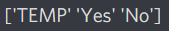
\includegraphics[width=.4\linewidth]{fig/fig2.png}
\caption{\label{figure2}
Unique values of self\_employed column.}
\end{figure}

\textbf{\emph{Part 3: Changing self\_employed "TEMP" values with "No"}}\bigbreak
We replaced this columns "TEMP" values with "No". We think that these values are left empty because they are not self employed.\bigbreak

\textbf{\emph{Part 4: Changing work\_interfere "TEMP" values with "Don't know"}}\bigbreak
We replaced this columns "TEMP" values with "Don't know". We think that these values are left empty because they are neutral.\bigbreak

\textbf{\emph{Part 5: Changing age values with median if age is smaller than 18 or greater than 100}}\bigbreak
Age column was containing illogical values such as, "9999" value. We found the median of this column, as shown in Figure 3, and changed these illogical values with it.\bigbreak

\begin{figure}[h]
\centering
    
\includegraphics[width=.3\linewidth]{fig/fig3.png}
\caption{\label{figure3}
Median of age column.}
\end{figure}

\textbf{\emph{Part 6: Creating age\_range feature}}\bigbreak
We decided to add new column named "age\_range" for visualization purposes. We categorized ages as "0-20", "21-30", "31-65", "66-100".\bigbreak

\textbf{\emph{Part 7: Decreasing gender values to male, female, trans}}\bigbreak
We reduced 49 different gender values, as shown in Figure 4, to male, female and trans.\bigbreak

\begin{figure}[h]
\centering
    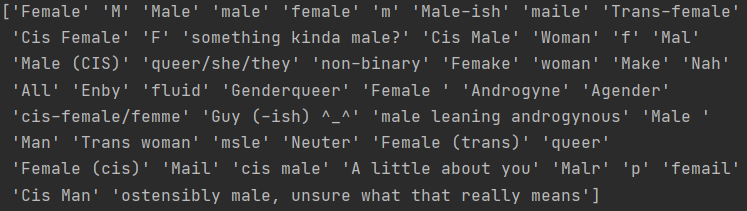
\includegraphics[width=.7\linewidth]{fig/fig4.png}
\caption{\label{figure4}
49 different gender values.}
\end{figure}

\subsubsection{Encoding dataset}
Our dataset was containing so many string values so we encoded our dataset with using LabelEncoder. Also, we scaled our age values with using MinMaxScaler because our age values were much different from other values in our dataset. Final version of out dataset after pre-processing can be seen at Figure 5.

\begin{figure}[h]
\centering
    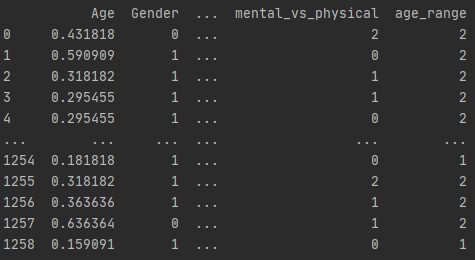
\includegraphics[width=.5\linewidth]{fig/fig5.png}
\caption{\label{figure5}
Dataset after pre-processing}
\end{figure}

\subsection{Data Visualization}
\subsubsection{Plotting charts for dataset visualization}
We wanted to understand our dataset better and to find the correlations between data so we have visualized some of them by using Seaborn and Matplotlib libraries. We used pie chart for distribution by gender as shown in Figure 6.a and histogram for distribution by age as shown in Figure 6.b.
When we examined the gender distribution in the dataset, we observed that men constituted the majority. Also, 25-35 age range appear to be more dense.

\begin{figure}[h]
\centering
\subfigure[Distribution by gender]{\centering
    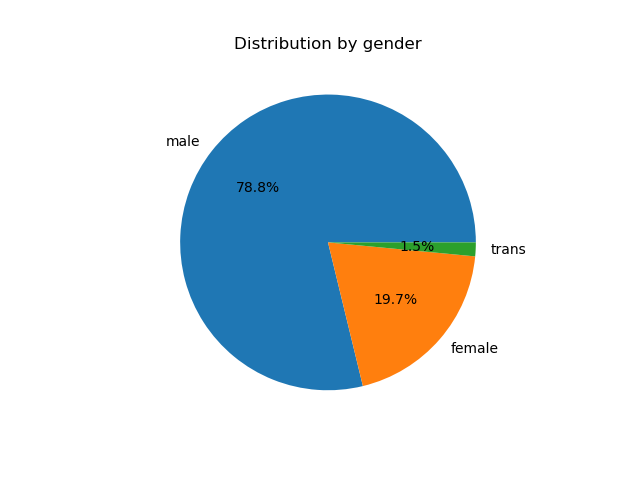
\includegraphics[width=.49\linewidth]{fig/fig6.png}
        \label{figure6}}
\subfigure[Distribution by age]{\centering
    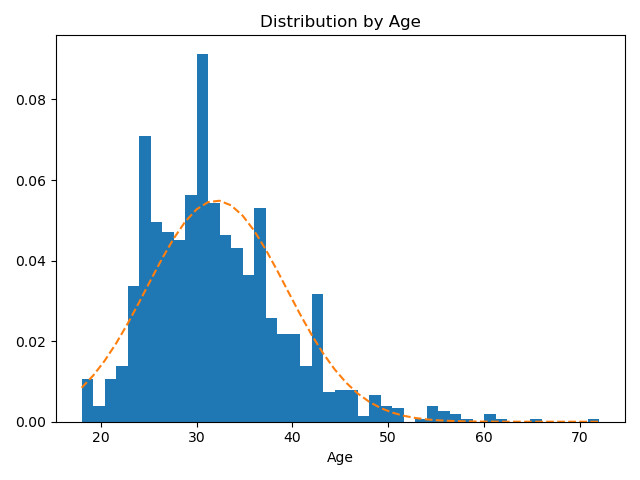
\includegraphics[width=.49\linewidth]{fig/fig7.png}
        \label{figure7}}
\caption{\label{}}
\end{figure}

We wanted to see the correlation between age range and mental health condition. We used barplot to show this with genders as shown in Figure 7. We see that male individuals have less mental health condition in all age groups than other individuals. Also we observed that there is a positive correlation between age and mental health condition.

\begin{figure}[h]
\centering
    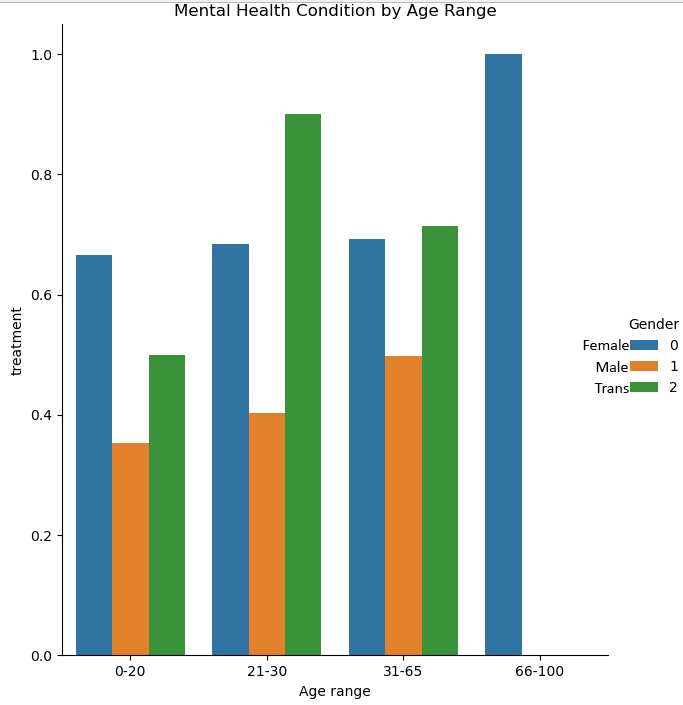
\includegraphics[width=.44\linewidth]{fig/fig8.png}
\caption{\label{figure8}
Mental health condition by age range}
\end{figure}

For family history and mental health condition correlation we used barplot again to show this with genders as shown in Figure 8. We see that family history has a great positive effect on mental health condition.\bigbreak
\begin{figure}[h]
\centering
    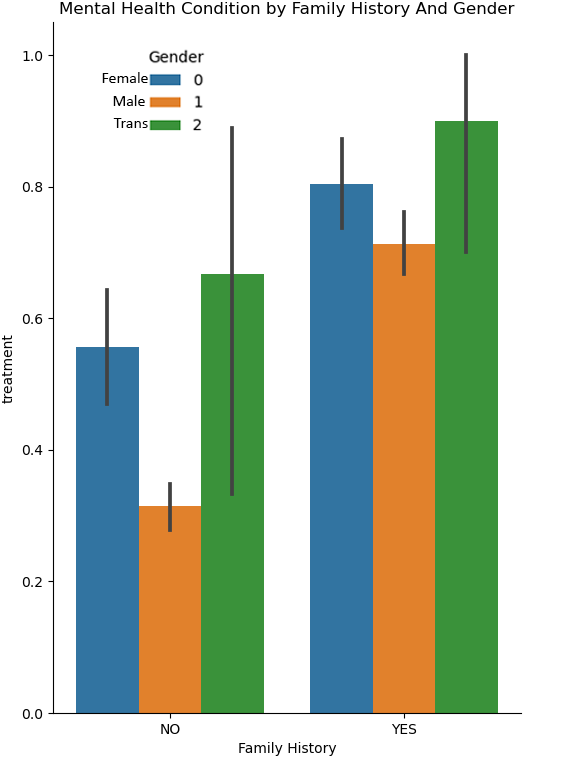
\includegraphics[width=.7\linewidth]{fig/fig9.png}
\caption{\label{figure9}
Mental health condition by family history}
\end{figure}



\subsection{Evaluating Models}
\subsubsection{Determining feature importance}
We made a ranking by using ExtraTreesClassifer in order to determine the features in our dataset that can affect the result the most. As a result of this ranking, we took the most important 9 features among 20 features, as shown in Figure 9, and trained our algorithms with these features.\bigbreak

\begin{figure}[h]
\centering
    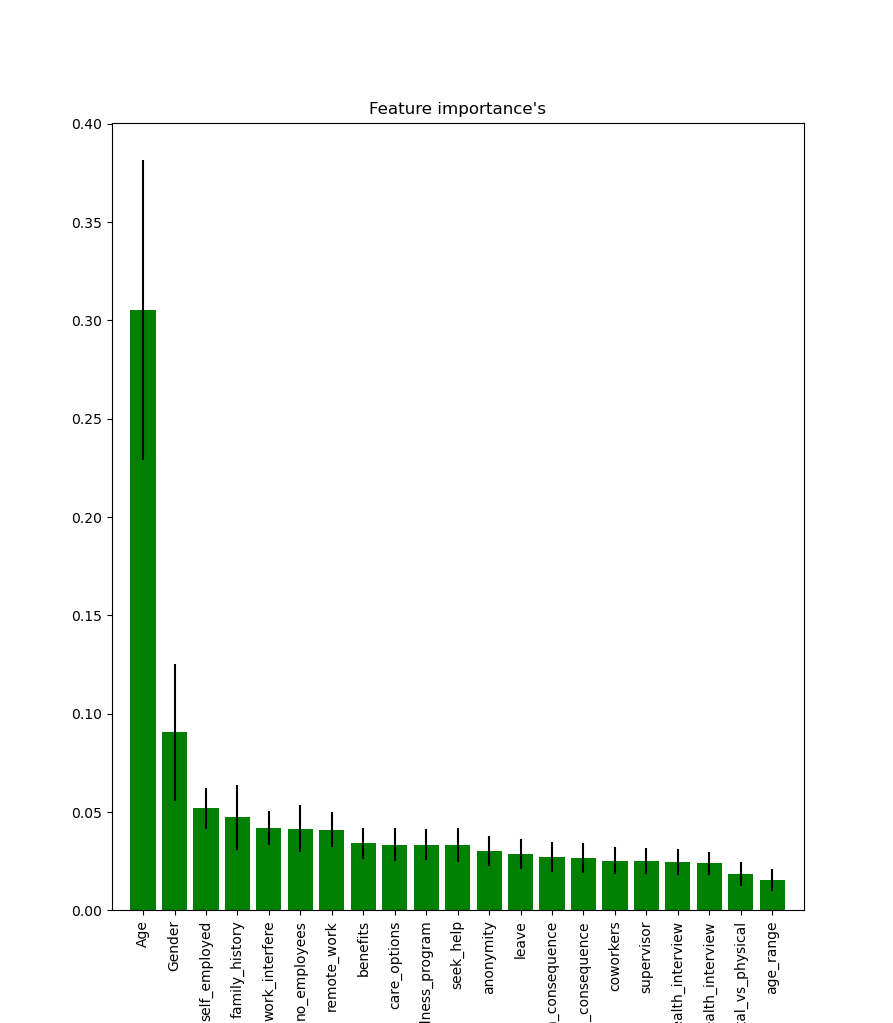
\includegraphics[width=.82\linewidth]{fig/fig10.png}
\caption{\label{figure10}
Feature importance's}
\end{figure}


\subsubsection{Applying algorithms}
In this section, before implementing the algorithms, we split our data set into 70 percent for training and 30 percent for testing. Then we created a confusion matrix function in addition to the output to better visualize the prediction results. We created heatmaps every one of them with using this function.\bigbreak

\textbf{\emph{Part 1: Logistic Regression}}\bigbreak
Logistic Regression is the appropriate regression analysis to conduct when the dependent variable is binary [3]. As a first task of applying algorithms part, we fitted our dataset into Logistic Regression and predicted. Then we found out accuracy with using accuracy\_score which is 79.3 percent. Heatmap of confusion matrix and results can be seen at Figure 10. \bigbreak

\begin{figure}[h]
\centering
{\centering
    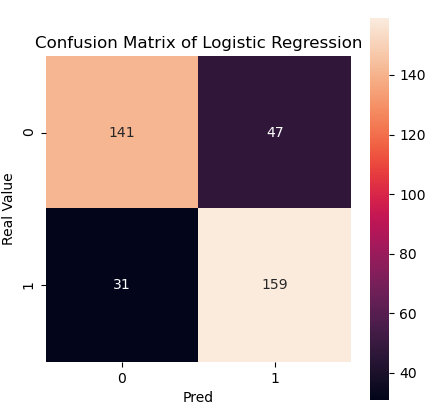
\includegraphics[width=.49\linewidth]{fig/fig_log2.png}
        \label{figure11}}
{\centering
    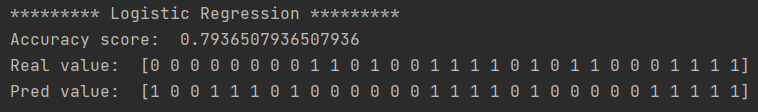
\includegraphics[width=.49\linewidth]{fig/fig_log1.png}
        \label{figure12}}
\caption{\label{Logistic Regression}Logistic Regression heatmap and results.}
\end{figure}

\textbf{\emph{Part 2: AdaBoost Classifier}}\bigbreak
AdaBoost algorithm is a Boosting technique that is used as an Ensemble Method in Machine Learning [4]. As a general principle, boosting algorithms try to obtain a strong learner by combining weak learners obtained in each iteration within the framework of certain rules. We fitted our dataset into AdaBoost Classifier and predicted. The default base estimator of AdaBoost is DecisionTreeClassifier. We created 50 weak learners with DecisionTreeClassifier and with learners, we made stronger predictions using AdaBoost. Then we found out accuracy with using accuracy\_score which is 81.7 percent. Heatmap of confusion matrix and results can be seen at Figure 10. \bigbreak

\begin{figure}[h]
\centering
{\centering
    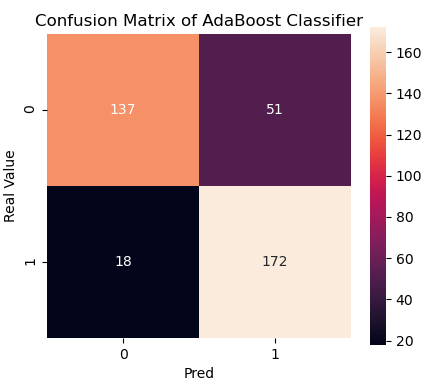
\includegraphics[width=.49\linewidth]{fig/fig_abc2.png}
        \label{figure13}}
{\centering
    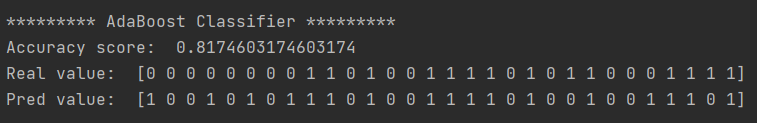
\includegraphics[width=.49\linewidth]{fig/fig_abc1.png}
        \label{figure14}}
\caption{\label{AdaBoost Classifier}AdaBoost Classifier heatmap and results.}
\end{figure}

\textbf{\emph{Part 3: KNeighbors Classifier}}\bigbreak
The K in the name of this classifier represents the k nearest neighbors, where k is an integer value specified by the user. Hence as the name suggests, this classifier implements learning based on the k nearest neighbors. The choice of the value of k is dependent on data. We made some tuning operations before we fit our dataset. We created a for loop with range of 1 to 53 and tried to find out the best n\_neighbors number by comparing every accuracy score. As a result, 17 was the best n\_neighbors number for our dataset. In this way, we increased the accuracy score from 76.6 percent to 79.3 percent. Heatmap of confusion matrix and results can be seen at Figure 12.\bigbreak

\begin{figure}[h]
\centering
{\centering
    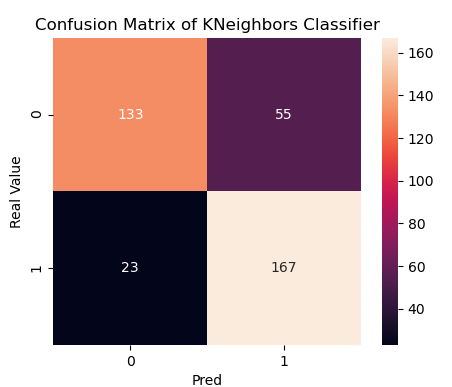
\includegraphics[width=.49\linewidth]{fig/fig_knc2.png}
        \label{figure15}}
{\centering
    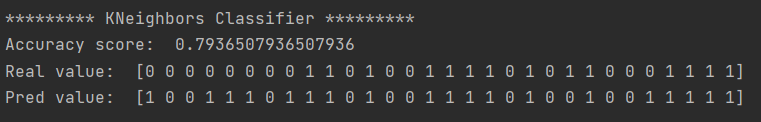
\includegraphics[width=.49\linewidth]{fig/fig_knc1.png}
        \label{figure16}}
\caption{\label{KNeighbors Classifier}KNeighbors Classifier heatmap and results.}
\end{figure}

\textbf{\emph{Part 4: Random Forest Classifier}}\bigbreak
As we know that a forest is made up of trees and more trees means more robust forest. Similarly, random forest algorithm creates decision trees on data samples and then gets the prediction from each of them and finally selects the best solution by means of voting. It is an ensemble method which is better than a single decision tree because it reduces the over-fitting by averaging the result[5]. We made some tuning operations before we fit our dataset. We created a for loop with range of 1 to 11 and tried to find out the best max\_depth number by comparing every accuracy score. As a result, 7 was the best max\_depth number for our dataset. In this way, we increased the accuracy score from 78.9 percent to 81.2 percent. Heatmap of confusion matrix and results can be seen at Figure 13. \bigbreak
\bigbreak
\bigbreak
\bigbreak
\bigbreak
\bigbreak
\bigbreak
\bigbreak
\bigbreak
\bigbreak
\bigbreak

\begin{figure}[h]
\centering
{\centering
    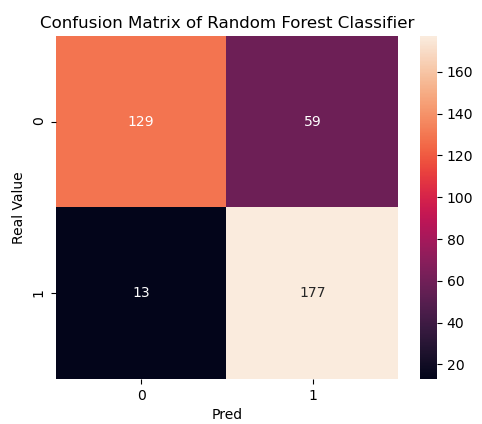
\includegraphics[width=.49\linewidth]{fig/fig_rfc2.png}
        \label{figure17}}
{\centering
    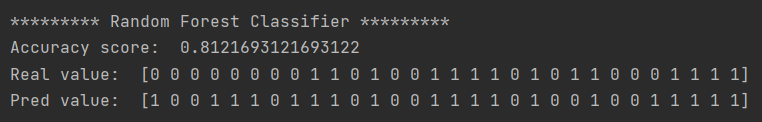
\includegraphics[width=.49\linewidth]{fig/fig_rfc1.png}
        \label{figure18}}
\caption{\label{Random Forest Classifier}Random Forest Classifier heatmap and results.}
\end{figure}

\textbf{\emph{Part 5: Bagging Classifier}}\bigbreak
Bagging classifier is an ensemble meta-estimator that fits base classifiers each on random subsets of the original dataset and then aggregate their individual predictions (either by voting or by averaging) to form a final prediction [6]. We made some tuning operations before we fit our dataset. We created a for loop with range of 4 random numbers and tried to find out the best max\_leaf\_nodes number by comparing every accuracy score. As a result, 99999 was the best max\_leaf\_nodes number for our dataset. In this way, we increased the accuracy score from 78.3 percent to 79.1 percent. Heatmap of confusion matrix and results can be seen at Figure 14.\bigbreak

\begin{figure}[h]
\centering
{\centering
    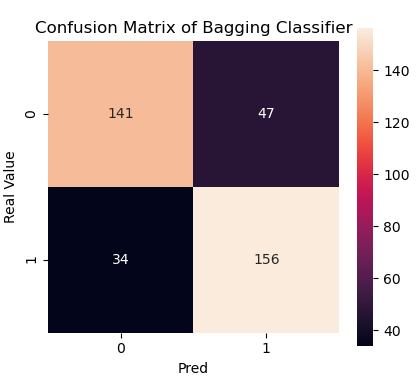
\includegraphics[width=.49\linewidth]{fig/fig_bag2.png}
        \label{figure19}}
{\centering
    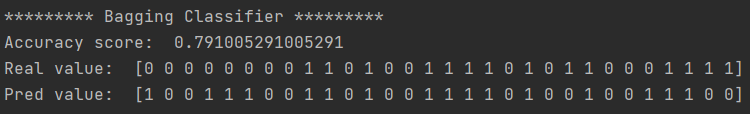
\includegraphics[width=.49\linewidth]{fig/fig_bag1.png}
        \label{figure20}}
\caption{\label{Bagging Classifier}Bagging Classifier heatmap and results.}
\end{figure}



\subsubsection{Comparison graph of algorithms by accuracy score}
After all tuning, fitting and predicting processes, although our algorithms give similar results, we have come to the conclusion that the most suitable algorithm for our data set is AdaBoost Classifier. Comparison graph can be seen at Figure 15.


\begin{figure}[h]
\centering
    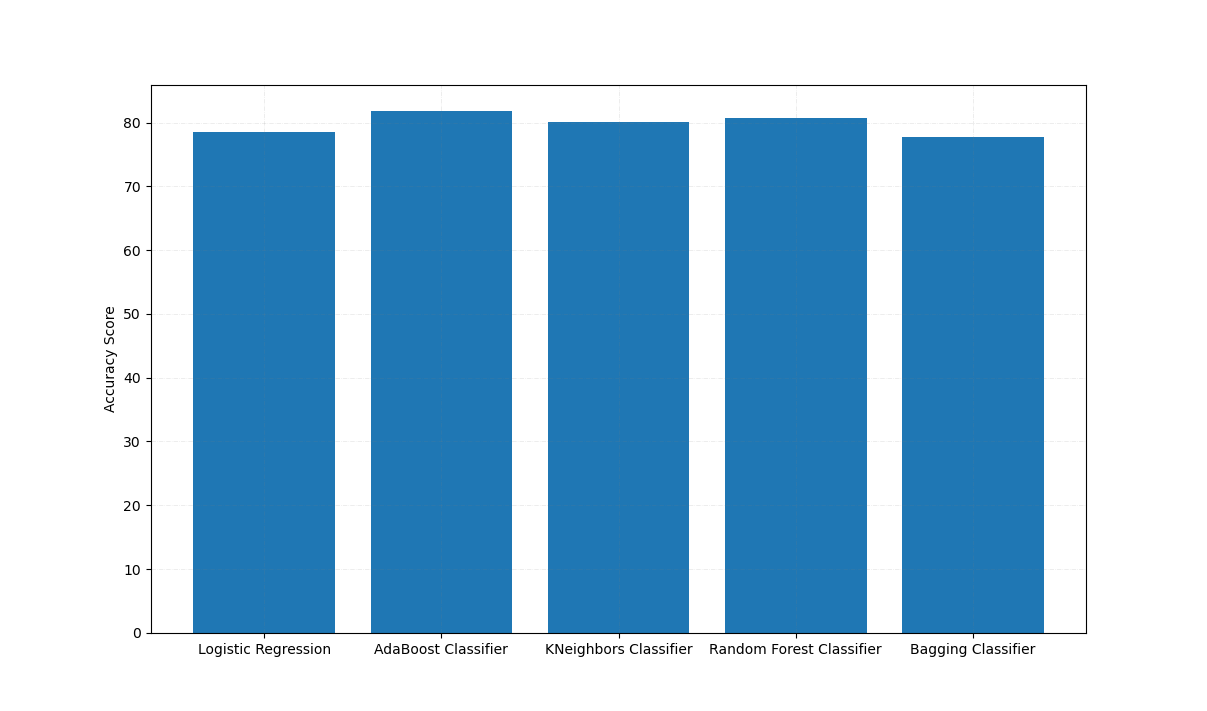
\includegraphics[width=1\linewidth]{fig/figgg.png}
\caption{\label{figure21}
Comparison graph of algorithms by accuracy score}
\end{figure}

\section{Conclusion}
To conclude, in this project, we tried to solve a simple real world problem by using supervised learning algorithms, such as Logistic Regression, AdaBoost Classifier, which is one of the data mining techniques. In order to analyze our dataset, we had to perform some operations (data cleaning, encoding, scaling etc.) because our dataset contained illogical data and missing values. These flaws could cause our analysis results to be different than expected. Then we made some visualizations and aimed to realize the correlations between the data and to have a general impression of the participants in our dataset.

After making our data ready for analysis, we first applied the Logistic Regression algorithm. As a result, we found an acceptable predict result. So was a single algorithm enough? We thought it would be better to try multiple algorithms to get higher prediction results. In addition to Logistic Regression, we used AdaBoost, KNeighbors, Random Forest and Bagging Classifiers. There are parameters in algorithms that directly affect our result. For example, we used the KNeighbors Classifier by changing the n\_neighbors parameter within a certain number range.

As a result of all these processes, we saw that AdaBoost Classifier gave the highest prediction result for use dataset among the five algorithms we applied.

\section{References}
[1] Stuart J. Russell, Peter Norvig (2010) Artificial Intelligence: A Modern Approach, Third Edition, Prentice Hall ISBN 9780136042594.\newline
[2] https://www.geeksforgeeks.org/data-preprocessing-in-data-mining/\newline
[3] https://www.statisticssolutions.com/what-is-logistic-regression/\newline
[4] https://medium.com/@sertacozker/boosting-algoritmalar%C4%B1-nas%C4%B1l-%C3%A7al%C4%B1%C5%9F%C4%B1r-edac1174e971 
\newline[5] https://www.tutorialspoint.com/machine\_learning\_with\_python/machine\_learning\_with\_python\newline\_classification\_algorithms\_random\_forest.htm\newline
[6] https://www.geeksforgeeks.org/ml-bagging-classifier/\newline
[7] Hinton, Geoffrey; Sejnowski, Terrence (1999). Unsupervised Learning: Foundations of Neural Computation. MIT Press. ISBN 978-0262581684.\newline
\nocite{*}
\end{document}

